\documentclass[UTF8]{ctexart}
%\setmainfont{Noto Sans CJK SC}
\usepackage{xeCJK}
\setCJKmainfont[BoldFont=Noto Sans S Chinese Bold Bold]{Noto Sans S Chinese Regular}
\usepackage{amsmath}
\usepackage{geometry}
\geometry{a4paper, left=2cm, right=2cm,top=2cm,bottom=2cm}
\usepackage{pifont}
%\ding{172}=\textcircled{1}
\usepackage{booktabs}
\usepackage{hyperref}
\usepackage{mathrsfs}
\usepackage{graphicx}
\usepackage{wrapfig}
\usepackage{float}
\usepackage[perpage]{footmisc}
\newcommand*{\dif}{\mathop{}\!\mathrm{d}}
\renewcommand{\thefootnote}{\ding{\numexpr171+\value{footnote}}}

\title{Part4 Diffraction}
\author{Xiao Liang}
\date{\today}


\begin{document}
	\maketitle
	\tableofcontents
	\numberwithin{equation}{section}
	%\CJKfontspec{Noto Sans Mono CJK SC}
	\CJKfontspec[BoldFont=Noto Sans S Chinese Bold Bold]{Noto Sans S Chinese Regular}
	
	\section{引言}
	衍射是一种光偏离直线传播的现象。衍射是波动现象的一个普遍特征,每逢波阵面的一部分(不论是声波、物质波还是光波)以某种方式受到阻碍时就会发生,如果在遇到障碍物(不论是透明的还是不透明的)的进程中,波阵面上的一个区域的振幅或位相受到改变,就会发生衍射。越过障碍物的波阵面的各个区段因干涉而引起特定的能量密度分布,叫做衍射图样。
	
	干涉和衍射之间并不存在实质性的物理差别,然而习惯上当 考虑的只是几个波的叠加时就说是干涉,而讨论大量的波的叠加时则说是衍射。
	
	惠更斯原理:一个波阵面上的每一个点都可以看成是次级球面子波的一个波源。于是波阵面或其任何一部分在空间的进一步传播应当可以预定出来,在任一特定时刻,假定波阵面的形状时次级子波的包络。但是,这一方法\textbf{忽略了各个次级子波的大部分,只保留了包络共有的那一部分}。由于这种不完善性,惠更斯原理不能说明衍射过程。
	
	菲涅耳通过加进来干涉概念解决了这一困难。相应的\textbf{惠更斯-菲涅耳原理}表述如下:在给定时刻,波阵面上的每一未被阻挡的点起着次级球面子波(频率与初级相同)波源的作用。障碍物外任一点上光场的振幅是所有这些子波的叠加(考虑它们的振幅和相对位相)。
	
	基尔霍夫利用老的光的弹性固体理论,用精致的分析使菲涅耳的假设得到论证,并且使惠更斯原理作为波动方程的一个精确结果,得到一个更精密的表述。然而,基尔霍夫理论本身也是一个近似,在波长充分小的时候才成立,而且需要求解偏微分方程,严格解只有在很少几种特殊情况下才能得到。除此之外,基尔霍夫理论只讨论标量波并且对光是一种横波矢量场这一事实毫无表示,然而它同实际符合得很好。
	
	\subsection{不透明障碍物}
	衍射可以被看成是\textbf{由于电磁波和某种物理障碍物的相互作用引起的}。
	
	一种可能的描述方法是,可以认为屏是一块连续媒介,即它的微观结构可以忽略。对于一块无吸收的金属薄片(不产生焦耳热,所以电导率是无穷大),我们可以写出金属中的麦克斯韦方程组和周围媒介中的麦克斯韦方程组,然后在边界上使二者匹配起来,于是可以得到一些非常简单的衍射问题的精确解。这时反射波和衍射波由薄片上的电流分布得出。
	
	在亚微观尺度考察这个屏,设想在入射波的电场作用下,各个原子的电子云开始振动起来。屏中的一个特定振子的振幅和位相由它周围的局部电场确定,而局部电场又是入射场和一切别的电子振子场的叠加。一张很大的不带孔的屏,都有一个明显的效应:在屏之后的区域内没有光场。靠近被照明一面的电子被入射光驱动而开始振动,它们发射辐射能,这个辐射能最后或被反射回来,或者以热的形式被材料吸收,或者二者兼而有之。不论是哪种情况,入射的初波和电子振子的场都将以这样的方式叠加,使得在屏后得任何一点上的光场为零。这看来是一种非常特殊的平衡,然而实际上并不是如此,如果初波没有完全被抵消,那么它将更深地进入屏材料内,激励更多电子产生辐射,这又会进一步使初波减弱,直到它最终消失为止(如果屏足够厚的话),不然还是可能透明。
	
	现在从屏的中央挖掉一个圆盘形小块,使得光通过此孔射出。在这块圆盘上均匀分布的振子同圆盘一起被去掉了,因而屏内剩下来的电子不再受它们影响。做一个近似的处理,\textbf{假定振子之间得相互作用实际上可以忽略},于是在孔后的区域中的场等于挖去圆盘之前所存在的场减去圆盘单独的贡献。在这一近似之下,衍射场可以被描绘成完全是由均匀分布在孔径区域上的一组假想的、不相互作用的振子产生的,这便是惠更斯-菲涅耳原理的实质。所以在距离衍射孔一段距离的情况下,这种假设是成立的,而如果要研究衍射孔附近的情况时,这种假设便失效了。
	
	\subsection{夫琅禾费衍射和菲涅耳衍射}
	两者的区别从现象上说就是:当观察屏远离衍射孔时,衍射图样会发生变化的便是菲涅耳衍射;反之,若只是会发生强度变化而形状不变的,便是菲涅耳衍射。菲涅耳衍射也叫做\textbf{近场衍射},而夫琅禾费衍射也叫做\textbf{远场衍射}。
	
	\subsection{模型:几个相干振子}
	考虑以下的模型:
	\begin{figure}[ht]
		\centering	
		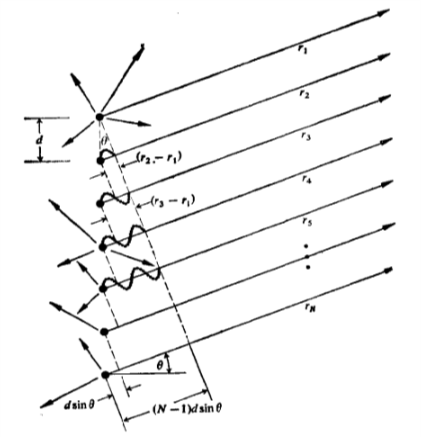
\includegraphics[width=14cm]{Diffraction_zhenzi.png}
		\caption{同相位的相干振子直线阵列}
		\label{figure_zhenzi}
	\end{figure}

	各个振子在一切方向甚至偏振方向都完全相同,暂且认为振子没有内在的位相差。所示的光线几乎全部平行,在很远的点$ P $相交,由于各个波走过差不多相等的距离,其振幅将基本上是相等的。在这个例子里不用考虑电场的矢量本性,考虑位相差可得:
	\begin{equation}
		E=E_{0}(r) e^{-i \omega t} e^{i k r_{1}}\left[1+e^{i k\left(r_{2}-r_{1}\right)}+e^{i k\left(r_{2}-r_{1}\right)}+\dots+e^{ik\left(r_{N}-r_{1}\right)}\right]\label{equ_E}
	\end{equation}
	
\noindent 相邻的点源之间的相位差为$ \delta=k_{0} \Lambda $,由于在折射率为$ n $的媒介中$ \Lambda =n d \sin \theta $,因而$ \delta= kd \sin \theta $由此可将\ref{equ_E}改写为:
\begin{equation}
	E=E_{0}(r) e^{-i \omega t} e^{i k r_{1}}\left[1+\left(e^{i \delta}\right)+\left(e^{i s}\right)^{2}+\left(e^{i d}\right)^{3}+\dots +\left(e^{i \delta}\right)^{N-1}\right]
\end{equation}

	考虑括号内的几何级数的值可以将场变为:
	\begin{equation}
	E=E_{0}(r) e^{-i \omega t} e^{i\left[k r_{1}+(N-1) \delta / 2\right]}\left(\frac{\sin N \delta / 2}{\sin \delta / 2}\right)
	\end{equation}
	
\noindent 定义$ R $为从振子直线的中央到$ P $点的距离,即:
\begin{equation}
\boldsymbol{R}=\frac{1}{2}(N-1) d \sin \theta+\boldsymbol{r}_{1}
\end{equation}

\noindent 则可以得到:
\begin{equation}
E=E_{0}(r) e^{i(k R-\omega)}\left(\frac{\sin N \delta / 2}{\sin \delta / 2}\right)
\end{equation}

\noindent 那么得到在远处排成直线阵列的$ N $个相干全同点源所产生的衍射图样内的通量密度分布为:
\begin{equation}
I=I_{0} \frac{\sin ^{2}(N \delta / 2)}{\sin ^{2}(\delta / 2)}
\end{equation}

\noindent 其中$ I_{0} $是任何一个波源到达$ P $点的通量密度,在$ N=0,I=0 $的情况下。考虑$ \theta $可得:
\begin{equation}
I=I_{0} \frac{\sin ^{2}[N(k d / 2) \sin \theta]}{\sin ^{2}[(k d / 2) \sin \theta]}\label{equ_I}
\end{equation}

	这个联合表达式\ref{equ_I}给出一系列尖锐的主峰,它们之间隔着小的辅峰,主极大出现在使得$ \delta=2 m \pi $的$ \theta_{m} $方向上,因为$ \delta = k d \sin \theta $,
	\begin{equation}
		d \sin \theta_{m}=m \lambda
	\end{equation}
	
\noindent 注意,在上式中,如果$ d<\lambda $,那么只有$ m=0 $或者只有零级主极大存在。如果考察彼此相隔为源自大小的距离的电子振子构成的理想化的线光源,可以预期,\textbf{光场中只有一个主极大}。

	考虑一个系统,在系统中相邻的振子间我们可以引入一个固有的相位差$ \varepsilon $。这时
	\begin{equation}
		\delta =k d \sin \theta + \varepsilon
	\end{equation}
	
\noindent 各个主极大将出现在新的角度上:
\begin{equation}
	d \sin \theta_{m} = m \lambda - \frac{\varepsilon}{k}
\end{equation}

\noindent 	如果我们只注意中央极大,那么只要调节$ \varepsilon $的值,就可以随意改变它的取向$ \theta_{0} $

	\begin{figure}[ht]
		\centering
		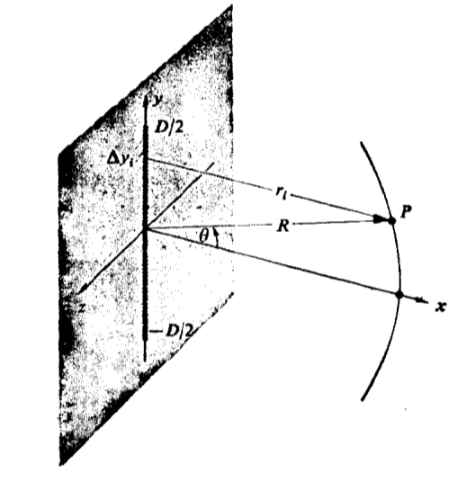
\includegraphics[width=12cm]{Diffraction_line_light.png}
		\caption{相干的线源}
		\label{figure_line}
	\end{figure}

	考虑一个电子振子的理想化的线波源(见图\ref{figure_line})。对于图\ref{figure_line},可以考虑一条宽度比$ \lambda $小得多的长狭缝被平面波照明时,惠更斯-菲涅耳原理的次级波源。每一个点发射一个球面子波,可以把这个子波写成:	
\begin{equation}
E=\left(\frac{\mathscr{E}_{0}}{r}\right) \sin (\omega t-k r)
\end{equation}

\noindent 它明显地显示出振幅对$ r $的反比关系,量$ \mathscr{E}_{0} $叫做\textbf{波源强度}。现在和图\ref{figure_zhenzi}不同的是,现在的波源很弱,而波源的个数$ N $非常之大,同时它们之间的距离则非常之小。阵列上的一小段(但有限长度)的$ \Delta y_{i} $,将包含$ \Delta y_{i} \left(\frac{N}{D}\right) $个源,其中$ D $是整个阵列的长度,假设分成$ M $段,则第$ i $段对$ P $点电场的贡献为:
\begin{equation}
E_{i}=\left(\frac{\mathscr{E}_{0}}{r_{i}}\right) \sin \left(\omega t-k r_{i}\right)\left(\frac{N \Delta y_{i}}{D}\right)
\end{equation}

\noindent 只要$ \Delta y_{i} $是这样小,使得其中振子的相对相位差可以忽略不计,因而它们的振幅直接以相长相加。令$ N $趋于无穷大,则可以把这个阵列编程连续地相干线源。

	在总输出有限的情况下,可以定义一个常数$ \mathscr{E}_{L} $为阵列的\textbf{单位长度的波源强度},即:
	\begin{equation}
	\mathscr{E}_{L} \equiv \frac{1}{D} \lim _{N \rightarrow \infty}\left(\mathscr{E}_{0} N\right)
	\end{equation}
	
\noindent $ M $个分段在$ P $点产生的总场强为可以通过求和得,而对于一个连续的线源,求和可以变成定积分:
\begin{equation}
	E=\mathscr{E}_{L} \int_{-D / 2}^{D / 2} \frac{\sin (\omega t-k r)}{r} d r \label{equ_line_E}
\end{equation}

\noindent 其中$ r=r(y) $。用来计算式\ref{equ_line_E}的近似方法取决于$ P $点相对于阵列的位置,由此可以区分夫琅禾费衍射和菲涅耳衍射两种情况。光学的相干线源作为一种物理实体现在还不存在,但可以作为一种数学工具来应用。

	\section{夫琅禾费衍射}
	\subsection{单缝}
	回到图\ref{figure_line},现在假设观察点离相干线源很远,再这样的情况下,$ r(y) $同它的中点值$ R $相差很少,因此量$ \frac{\mathscr{E}_{L}}{R} $在$ P $点之值基本上对于所有线源$ \dif y $都是常数。由式\ref{equ_line_E}可得光源的微分线源在$ P $产生的场为:
	\begin{equation}
	\dif E=\frac{\mathscr{E}_{L}}{R} \sin (\omega t-k r) \dif y\label{equ_E_dif}
	\end{equation}
	
	其中,$\frac{\mathscr{E}_{L}}{R} \dif y$是波的振幅。由于位相对$ r(y) $的变化要比振幅敏感得多,因此对它作近似时需要非常小心。对$ r(y) $展开,可以得到:
	\begin{equation}
	r=R-y \sin \theta+\left(y^{2} / 2 R\right) \cos ^{2} \theta+\cdots
	\end{equation}
	
	可以略去第三项的条件是:它对相位的贡献甚至当$ y=\pm \frac{D}{2} $也不大,即$ \left(\frac{\pi D^{2}}{4 \lambda R}\right) \cos^{2} \theta $必须可以忽略不计。当$ R $足够大的时候,这个条件可以对一切$ \theta $值成立,这就是\textbf{夫琅禾费条件}。代入\ref{equ_E_dif}并积分可得:
	\begin{equation}
	E=\frac{\mathscr{E}_{L}}{R} \int_{-D / 2}^{+D / 2} \sin \left[\omega t-k(R-y \sin \theta)\right] \dif y
	\end{equation}
	
\noindent 得到
\begin{equation}
E=\frac{\mathscr{E}_{L} D}{R} \frac{\sin [(k D / 2) \sin \theta]}{(k D / 2) \sin \theta} \sin (\omega t-k R)
\end{equation}

\noindent 为简化上式,令
\begin{equation}
\beta \equiv \frac{k D}{2} \sin \theta
\end{equation}

\noindent 因此
\begin{equation}
E=\frac{\mathscr{E}_{L} D}{R}\left(\frac{\sin \beta}{\beta}\right) \sin (\omega t-k R)\label{equ_E_single_feng}
\end{equation}

\noindent 考虑到最便于测量的是辐照度$I(\theta)=\left\langle E^{2}\right\rangle$(这里照常忽略常数因子),于是
\begin{equation}
I(\theta)=\frac{1}{2}\left(\frac{\mathscr{E}_{L} D}{R}\right)^{2}\left(\frac{\sin \beta}{\beta}\right)^{2}
\end{equation}

\noindent 容易得到:
\begin{equation}
I(\theta)=I(0)\left(\frac{\sin \beta}{\beta}\right)^{2}
\end{equation}

\noindent 这就是在夫琅禾费近似下一个理想化的相干光源产生的辐照度。结果如下:
\begin{figure}[ht]
	\centering
	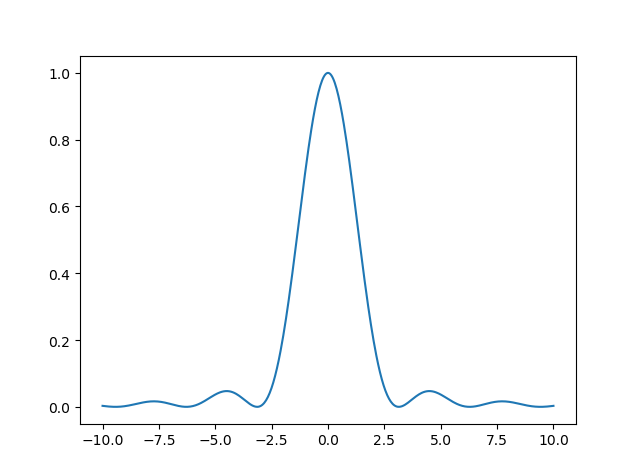
\includegraphics[width=12cm]{Diffraction_fulang_I.png}
	\caption{理想化的相干线光源产生的辐照度在夫琅禾费近似下和$ \beta $的关系曲线}
	\label{figure_fulang_I}
\end{figure}

\noindent 注意,由于$ \beta=\left(\frac{\pi D}{\lambda}\right) \sin \theta $,当$ D\gg \lambda $时,辐照度随着$ \theta $离开零而极速地减弱(这点在图$ \ref{figure_fulang_I} $中没有体现)。一个比较长的相干线源($ D \gg \lambda $)可以看作一个主要在$ \theta=0 $方向上辐射的点发射体,而若相干线源处于相反的情况下,则辐照度对一切$ \theta $都是常数,线源也就类似于发射球面波的一个点源了。

	现在讨论狭缝或者长而窄的矩形孔的夫琅禾费衍射。一个这样的孔地典型宽度是几百个波长,长度是几个厘米。考虑将这个狭缝分成一系列平行于$ y $轴的微分长条,每一个长条都是一个长的相干线源,可以换成在z轴上的一个点发射体。实际上,每个这样的发射体在xz平面上辐射一个圆形波。这是合理的,因而狭缝很长,因而出射波阵面在狭缝方向实际上并未受到阻碍。因此,在平行于狭缝两端边界的方向上几乎没有什么衍射。这样,这个问题就化为求沿着缝宽方向(z轴)排列的无穷多个电源在xz平面上产生的场的问题。在这种情况下积分又等价于一个相干线源,即
	\begin{equation}
	I(\theta)=I(0)\left(\frac{\sin \beta}{\beta}\right)^{2}
	\end{equation}
	
\noindent 如果
\begin{equation}
\beta=(k b / 2) \sin \theta
\end{equation}

\noindent 现在$ \theta $是从xy平面量起的。注意到,现在线源很短,$ D=b $,因此$ \beta $不大,虽然辐射度减弱地很快,但高次的辅峰仍然可以被观察到。
\begin{figure}[ht]
	\centering
	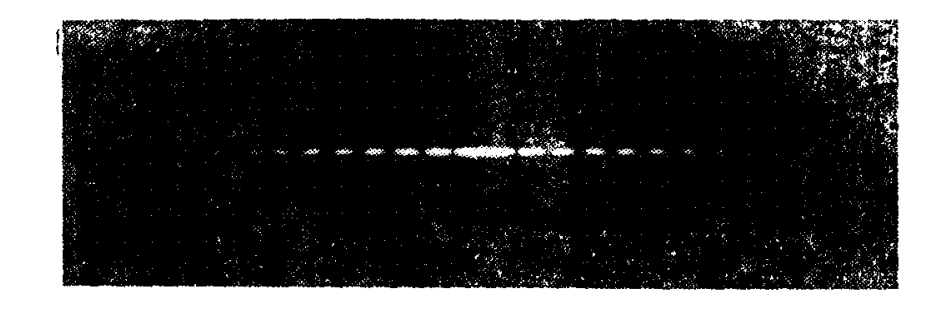
\includegraphics[width=12cm]{Diffraction_xiafeng.png}
	\caption{单(铅直)狭缝在点光源照明下的衍射图样}
	\label{figure_xiafeng}
\end{figure}

	现在来计算$ I(\beta) $的极值出现的位置。理论上应该出现在$ \frac{\dif I}{\dif \beta}=0 $的位置上,即
	\begin{equation}
	\frac{d I}{d \beta}=I(0) \frac{2 \sin \beta(\beta \cos \beta-\sin \beta)}{\beta^{3}}=0
	\end{equation}
	
\noindent 容易得到一类解为
\begin{equation}
\beta=\pm \pi, \pm 2 \pi, \pm 3 \pi, \cdots
\end{equation}

\noindent 另一类解由超越方程$ \beta \cos \beta-\sin \beta =0 $确定,由图解法或其他数值方法可以得到。

	留意:惠更斯-菲涅耳原理的弱点之一是,它没有对在各个次级子波的表面上振幅随角度的变化给予正当的考虑,在涉及到\textbf{倾斜因子}时这一点尤为明显。在夫琅禾费衍射中,从孔道观察平面的距离时如此之大,因此不必考虑这一效应,在$ \theta $始终很小的情况下。
	
	考虑通量密度曲线,由于$ \beta=\left(\frac{\pi b}{\lambda}\right) \sin \theta $和$ \lambda $有关,所以如果光源发射白光,那么随着$ \theta $的增大,高级极大就会显示出向红色过渡的颜色序列,各个不同颜色的光分量由它自己的极小和辅极大,其角位置由波长决定。这使得只有在$ \theta=0 $附近的区域,所有各种成分的颜色才会重叠在一起而得出白光。
	
	\begin{figure}[ht]
		\centering
		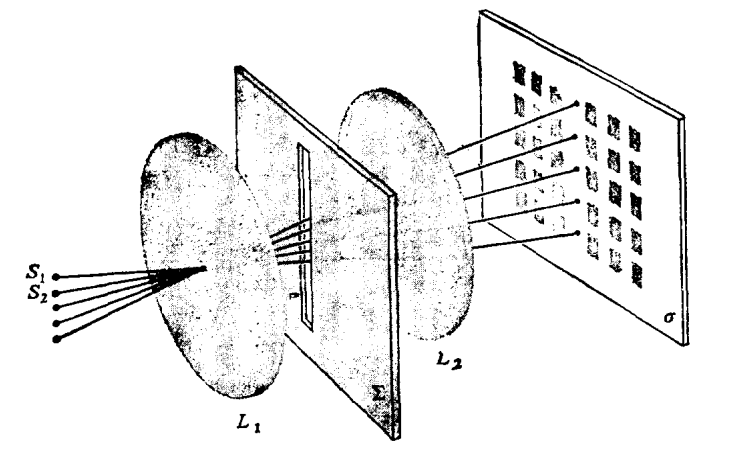
\includegraphics[width=12cm]{Diffraction_non_relevant.png}
		\caption{用不相干线源产生的单缝图样}
		\label{figure_non_relevant}
	\end{figure}

	考虑把光源$ S $换成一个非相干的线光源,它平行于狭缝,并位于准直透镜$ L_{1} $的焦面上,则图样将展宽成一组光带,线光源上的任意一点都产生一组独立的衍射图样,每个独立的图样都相对于其他的图样在$ y $方向平移。因此如果没有衍射屏,线光源的象会是平行于原来狭缝的一条直线;有衍射屏时,这条直线会扩展开,如同点源$ S $的象那样(图\ref{figure_non_relevant})。
	
	\subsection{双缝}
	不论狭缝的位置在哪里,只要取向不变且所做的近似成立,衍射图样实际上就是以透镜轴为中心,并且具有完全相同的形状和位置。
	\newpage
	\begin{figure}[ht]
		\centering
		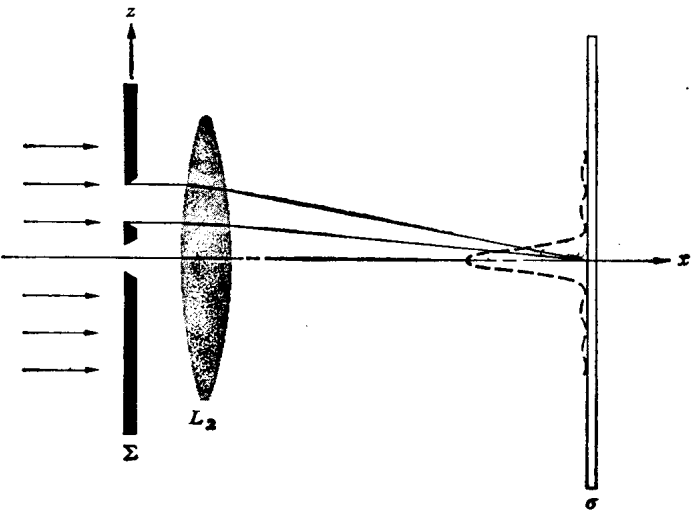
\includegraphics[width=12cm]{Diffraction_double_feng.png}
		\caption{双缝装置}
		\label{figure_double_feng}
	\end{figure}

\noindent 平行于透镜轴的一切光线都会聚到$ L_{2} $的第二焦点上,于是它就是$ S $的象,即衍射图样的中心。假设我们有两条长狭缝,每个狭缝自身在观察屏上将产生相同的单缝衍射图样。来自两条狭缝的贡献在观察屏上的任何一点重叠在一起时,虽然每个贡献的振幅必须基本上相等,但它们的相位可以差别很大,由于每个狭缝上的次级波源是同一初波激发的,结果产生的子波将是相干的,因此必定会发生干涉。所得到的通量密度将是由单缝衍射图样所调至的快速变化的双缝干涉系统的组合体。

	仿照单缝时的光扰动表达式,在夫琅禾费近似下,可以得到对电场的总贡献是:
	\begin{equation}
	E=C \int_{-b / 2}^{b / 2} F(z) \dif z+C \int_{a-b / 2}^{a+b / 2} F(z) \dif z
	\end{equation}
	
\noindent 其中$F(z)=\sin [\omega t-k(R-z \sin \theta)]$,常数振幅因子$ C $是沿$ z $轴单位长度上的次级光源强度(假定它在每个孔上都与$ z $无关)除以$ R $,$ R $是从原点到$ P $的距离取为常数。由于我们只关心相对通量密度,它的值意义不大。积分上式可得:
\begin{equation}
E=b C\left(\frac{\sin \beta}{\beta}\right)[\sin (\omega t-k R)+\sin (\omega t-k R+2 \alpha)]
\end{equation}

\noindent 其中$\alpha \equiv(k \alpha / 2) \sin \theta$,和前面一样$\beta \equiv(k b / 2) \sin \theta$,这正是每一狭缝在$ P $点产生的两个形如式\ref{equ_E_single_feng}那样的场之和。进一步简化可以得到:
\begin{equation}
E=2 b C\left(\frac{\sin \beta}{\beta}\right) \cos \alpha \sin (\omega t-k R+\alpha)
\end{equation}

\noindent 对上式平方并对比较长的时间间隔求平均,可以得到辐照度:
\begin{equation}
I(\theta)=4 I_{0}\left(\frac{\sin ^{2} \beta}{\beta^{2}}\right) \cos ^{2} \alpha
\end{equation}

\noindent $ I_{0} $是每条狭缝对通量密度的贡献,而$ I(0)=4 I_{0} $则是总的通量密度。因子4来源于以下事实:电场的振幅是当一条狭缝被遮住时那一点上应有的振幅的两倍。

	\subsection{多缝衍射}
	类似双缝衍射的方式对所有狭缝的贡献进行叠加,由于仍然使用夫琅禾费条件,孔的构形必须使得所有狭缝都靠近原点,近似条件($ r=R-z \sin \theta $)对每一条狭缝均成立,由此可以得到:
	\begin{equation}
	E_{j}=b C\left(\frac{\sin \beta}{\beta}\right) \sin (\omega t-k R+2 \alpha j)
	\end{equation}
	
\noindent 最后的结果如下:
\begin{equation}
E=\sum_{j=0}^{N-1} E_{j}=b C\left(\frac{\sin \beta}{\beta}\right)\left(\frac{\sin N \alpha}{\sin \alpha}\right) \sin [\omega t-k R+(N-1) \alpha]
\end{equation}

\noindent 通量密度分布函数为:
\begin{equation}
I(\theta)=I_{0}\left(\frac{\sin \beta}{\beta}\right)^{2}\left(\frac{\sin N \alpha}{\sin \alpha}\right)^{2}
\end{equation}

	\subsection{矩形孔}
	对于一个孔的夫琅禾费衍射,可以将孔内的一个微分面元$ \dif S $想象成由相干的次级点光源覆盖着,但是$ \dif S $比$ \lambda $小得多,所以它们对$ P $点的全部贡献保持同相,因而干涉相长。如果$ \mathscr{E}_{A} $是单位面积的源强,\textbf{假定它在整个孔上是常数},由此可以得到:
	\begin{equation}
	\dif E=\left(\frac{\mathscr{E}_{A}}{r}\right) e^{i(\omega t-k \tau)} \dif S
	\end{equation}
	
\noindent 的实部或者虚部。从$ \dif S $到$ P $的距离是
\begin{equation}
r=\left[X+(Y-y)^{2}+(Z-z)^{2}\right]^{1 / 2}
\end{equation}

\noindent 可对其进行展开,利用$ R=\sqrt{X^{2}+Y^{2}+Z^{2}} $可以得到:
\begin{equation}
	r=R\left[1+\left(y^{2}+z^{2}\right) / R^{2}-2(Y y+Z z) / R^{2}\right]^{1 / 2}
\end{equation}

\noindent 在远场情况下,$ R $比孔的线度要大得多,同时无论如何$ \theta $都可以保持很小,不必对辐射体的方向性作任何考虑,于是
\begin{equation}
r=R\left[1-2(Y y+Z z) / R^{2}\right]^{1 / 2}
\end{equation}

\noindent 在二项式中只保留前两项,同时考虑矩形衍射孔的情况,可以得到:
\begin{equation}
E=\frac{\mathscr{E}_{A} e^{i(\omega t-k R)}}{R} \int_{-b / 2}^{+b / 2} e^{i k Y y / R} \dif y \int_{-a / 2}^{+a / 2} e^{i k Z z / R} \dif z
\end{equation}

\noindent 其中$ \dif S= \dif y \dif z $。令$ \beta^{\prime} \equiv \frac{k b Y}{2 R} $及$ \alpha^{\prime} \equiv \frac{k a Z}{2 R} $,可以得到:
\begin{equation}
	E=\frac{A \mathscr{E}_{A} e^{\lambda \left(\omega t- k R\right)}}{R} \left(\frac{\sin \alpha^{\prime}}{\alpha^{\prime}}\right)\left(\frac{\sin \beta^{\prime}}{\beta^{\prime}}\right)
\end{equation}

\noindent 其中$ A $是孔的面积,可以得到:
\begin{equation}
I(Y, Z)=I(0)\left(\frac{\sin \alpha^{\prime}}{\alpha^{\prime}}\right)^{2}\left(\frac{\sin \beta^{\prime}}{\beta^{\prime}}\right)^{2}
\end{equation}

	\subsection{圆孔}
	利用一个任意孔在$ P $点所产生的光扰动表达式
	\begin{equation}
		E=\frac{\mathscr{E}_{A} e^{i\left(\omega t- k R\right)}}{R} \int \int e^{ik \frac{\left(Y y+ Z z\right)}{R}} \dif S
	\end{equation}
	
\noindent 对于一个圆孔,考虑使用球坐标,由于问题是完全轴对称的,其解一定与$ \Phi $无关,可以令$ \Phi=0 $来求解。注意二重积分中与变量$ \phi $有关的部分$\int_{0}^{2^{\pi}} e^{i(k \rho q / R) \cos \phi} d \phi $可以化为零阶的(第一类)\textbf{贝塞尔函数},即
\begin{equation}
J_{0}(u)=\frac{1}{2 \pi} \int_{0}^{2 \pi} e^{i u \cos v} d v
\end{equation}

\noindent 注意坐标变换关系如下:
\begin{equation}
	\begin{aligned}
	z&=\rho \cos \phi, y=\rho \sin \phi\\
	Z&=q \cos \Phi, Y=q \sin \Phi
	\end{aligned}
\end{equation}

	由此我们可以得到:
	\begin{equation}
	E(t)=\frac{\mathscr{E}_{A} e^{i(\omega t-k R)}}{R} 2 \pi a^{2}(R / k a q) J_{1}(k a q / R)
	\end{equation}
	
\noindent 辐照度为:
\begin{equation}
I=\frac{2 \mathscr{E}_{A}^{2} A^{2}}{R^{2}}\left[\frac{J_{1}(k a q / R)}{k a q / R}\right]^{2}
\end{equation}

\noindent 由于$ \sin \theta= \frac{q}{R} $,辐射度可以写作:
\begin{equation}
I(\theta)=I(0)\left[\frac{2 J_{1}(k a \sin \theta)}{k a \sin \theta}\right]^{2}
\end{equation}

	中心最亮的那个斑点被称为\textbf{爱里斑},爱里斑被一个暗环包围着,暗环相当于函数$ J_{1}(u) $的第一个零点。查表可得头一个暗环半径,也即爱里斑的半径为:
	\begin{equation}
		q_{1}=1.22 \frac{R \lambda}{2 a}
	\end{equation}
	
\noindent 对于一个聚焦到屏上的透镜,焦距$ f \approx R $,因此
\begin{equation}
	q_{1} \approx 1.22 \frac{f \lambda}{D}
\end{equation}

\noindent 其中,$ D=2a $是孔的直径。

\subsection{成像系统的分辨率}
	设想我们有某种透镜系统,它对一个扩展体成像。如果物体是自发光体,可以认为它是由非相干光源阵列过程的;而在反射光中看到的物体,它的各个散射点之间肯定将呈现某种相位相关性。当点光源实际上不是相干的,透镜系统将形成这样的一个像:它又部分重叠的、但是独立的爱里斑图样的分布组成。在像差已经做到可以忽略的、非常好的透镜中,由衍射引起的每个像点的扩展就代表对象的质量的最终限制。
	
	考虑远处的两个等辐照度的非相干点光源,例如通过望远物镜看到的两个星,这里入射光瞳就相当于衍射孔。爱里斑的直径为$ q_{1}= 1.22\frac{f \lambda}{D} $,如果$ \Delta \theta $是对应的角的大小,则$ \Delta \theta =1.22 \frac{\lambda}{D} $,因为$ \frac{q_{1}}{f}=\sin \Delta \theta \approx \Delta \theta $.\ 每个星的爱里斑将在它的几何像点周围、半角宽度$ \Delta \theta $内扩展开,如果两个星的角距离$ \Delta \varphi \gg \Delta \theta $,那么两个像将是截然分开并且容易分辨的。采用瑞利判据:\textbf{如果一个爱里斑的中心落在另一颗星的第一个极小时,便认为这两颗星刚刚可以分辨}。这个最小可分辨角间隔或角分辨极限是
	\begin{equation}
	(\Delta \varphi)_{\min }=\Delta \theta=\frac{1.22 \lambda}{D}
	\end{equation}
	
\noindent 如果$ \Delta l $是两个像从中心到中心的距离,则\textbf{分辨极限}是
	\begin{equation}
	(\Delta l)_{\min }=\frac{1.22 f \lambda}{D}
	\end{equation}
	
\noindent 一个成像系统的\textbf{分辨本领}一般被定义为$ \frac{1}{(\Delta \varphi)_{min}} $或者$ \frac{1}{\Delta l_{min}} $

	要减小两个像之间的最小可分辨间隔,一个办法是\textbf{使波长变小},在显微镜中使用紫外线而不用可见光,就能够观察到更精细的细节。电子显微镜利用的等效波长约为可见光波的$ 10^{-4} \rightarrow 10^{-5} $,这使得它能够考察在可见光频段由于衍射效应将会完全模糊的物体。另一个方面也可以\textbf{增大物镜或反射镜的直径},这样做除了收集到更多的入射辐射之外,还将使所产生的爱里斑更小,因而得到一个轮廓更清楚、更明亮的像。
	
	Sparrow 极限是关于分辨本领的一个更适当的判据,它利用了瑞利极限上相邻两个峰之间有一个中央极小或鞍点。进一步减小两个点光源之间的距离,将会使中央凹陷越来越浅,最终就会消失,同这种情况对应的角间隔就是Sparrow极限。
	
	\subsection{衍射光栅}
	
	衍射元件(不论是透光孔还是不透光的障碍物)的重复阵列能够使一个出射波的相位、振幅或者两者都产生周期性的交替变化,这种重复阵列叫做\textbf{衍射光栅}。
	
	最早的光栅是多缝装置,通常由绕在作支架用的两个平行螺丝之间的细线栅组成。一个波阵面在通过这样一个系统时,碰到交替的透明和不透明的区域,因而其振幅受到调制,因此,一个多缝结构叫做\textbf{投射振幅光栅}。投射光栅另一种更为常见的形式是在平面明净的玻璃上刻上平行的凹槽,各条刻痕是散射光的一个光源,它们合在一起就构成一个有规则的平行的线光源阵列。但光栅是完全透明的,因此振幅调制可以忽略不计时,光栅上的光学厚度的有规则变化产生\textbf{相位调制},这就得到了所谓的\textbf{透射位相光栅}。
	
	在从这种光栅上反射时,由不同的周期性表面特征所散射的光以一定的相位关系到达某一点P.\ 反射后所产生的干涉图样同投射所产生的干涉图样非常相似。特别设计的、以这种方式工作的光栅叫做\textbf{反射位相光栅}。
	
	如果垂直地通过一块投射光栅观察远处的平行的线光源,那么眼将起着形成衍射图样的聚焦透镜的作用,通过之前的计算可以得到
	\begin{equation}
		a \sin \theta_{m}= m \lambda
	\end{equation}
	
\noindent 这是垂直入射时的\textbf{光栅公式},$ m $的值规定了各级主极大的值。对于一个光谱范围很宽而且连续的光源,零级像对应于光源的不偏折的白光像。光栅公式和波长有关,因此对于$ m \neq 0 $的任何值,光源被展开成一条连续的光谱,由微弱的辅峰所占的区域显得是没有任何光的暗带。

	考虑普遍的斜入射的情况。对于投射光栅和反射光栅两种情况,光栅公式都变成
	\begin{equation}
	a\left(\sin \theta_{m}-\sin \theta_{i}\right)=m \lambda
	\end{equation}
	
\noindent 这个表达式不论透射光栅本身的折射率是多大都同样适用。

	这类普通的光栅有个缺点,便是大部分的光强都集中在零级之中,这会导致很大程度的浪费。因此,绝大多数的现代光栅是\textbf{闪耀光栅}的变种,这种光栅本质是形状可控制的沟槽,可以把能量从无用的零级谱转移到高级谱上去。非零的各级的角位置(即$ \theta_{m} $值)由$ a,\lambda $和更直接相关的$ \theta_{i} $决定。但是$ \theta_{i},\theta_{m} $是从光栅平面的法线量起,而不是相对于单个沟槽的表面来量的。另一方面,单个沟槽表面衍射图样中的峰的位置则对应于每个刻槽的表面的镜面反射,它由\textbf{闪耀角}$ \gamma $(即斜面倾角)决定,并且可以独立于$ \theta_{m} $而加以改变。相邻的两个槽面之间在入射光的反方向上的光程差为:
	\begin{equation}
		\Delta = 2d \sin \gamma=\lambda_{B}
	\end{equation}
	
\noindent 可以推得,波长为$ \lambda_{B} $的1级光谱就在所考察的方向上,并且与单槽面衍射的零级主极大重合,这一级光谱将获得最大的光强度,因而$ \lambda_{B} $被称为1级闪耀波长。
\begin{figure}[H]
	\centering
	\begin{minipage}[t]{0.48 \textwidth}
		\centering
		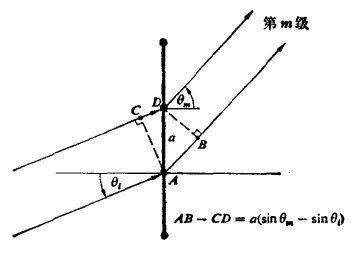
\includegraphics[width=6cm]{Diffraction_shan_t.png}
		\caption{透射光栅}
		\label{figure_shan_t}
	\end{minipage}
	\begin{minipage}[t]{0.48 \textwidth}
		\centering
		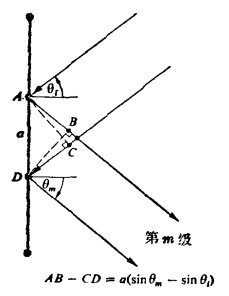
\includegraphics[width=6cm]{Diffraction_shan_r.png}
		\caption{反射光栅}
		\label{figure_shan_r}
	\end{minipage}
\end{figure}

	\subsection{光栅光谱学}
	假定有一个无穷窄的非相干光源,一条出射光谱线的有效宽度可以定义为一个主峰两侧的零点之间的角距离,即$ \Delta \alpha = \frac{2 \pi}{N} $.\ 在斜入射时,可以把$ \alpha $重新定义为$ \frac{k a}{2} (\sin \theta - \sin \theta_{i}) $,因而$ \alpha $的一个有限改变由下式给出:
	\begin{equation}
	\Delta \alpha=(k a / 2) \cos \theta(\Delta \theta)=2 \pi / N
	\end{equation}
	
\noindent 其中入射角为常数,故$ \Delta \theta_{i}=0 $。由上式可知,即使入射光是单色光,一个谱线也具有角宽度
\begin{equation}
\Delta \theta=2 \lambda /\left(N a \cos \theta_{m}\right)
\end{equation}

\noindent 它属于\textbf{仪器展宽}。

	另一个重要的量是一定的波长差所对应的角位置之差,\textbf{角色散}定义为
	\begin{equation}
	\mathscr{D} \equiv d \theta / d \lambda
	\end{equation}
	
\noindent 对光栅公式求微商可得:
\begin{equation}
\mathscr{D}=m / a \cos \theta_{m}
\end{equation}

\noindent 这表明,随着光谱级的增大,两条不同频率的谱线之间的角间隔也将增大。

	当两条谱线之间的波长差足够小以致互相重叠时,所得到的峰就变得不明确了。定义光谱仪的色分辨本领为
	\begin{equation}
	\mathscr{R} \equiv \lambda /(\Delta \lambda)_{\min }
	\end{equation}
	
\noindent 其中$ (\Delta \lambda)_{min} $是可分辨的最小波长差或\textbf{分辨极限},$ \lambda $是平均波长。两个等通量密度条纹可以分辨的瑞利判据要求:一个条纹的主极大同另一个条纹的第一极小相重合。如下图所示,在这一分辨极限下,角间隔是线宽的一半,故
\begin{equation}
(\Delta \theta)_{\min }=\lambda / N a \cos \theta_{m}
\end{equation}

	\begin{figure}[ht]
		\centering
		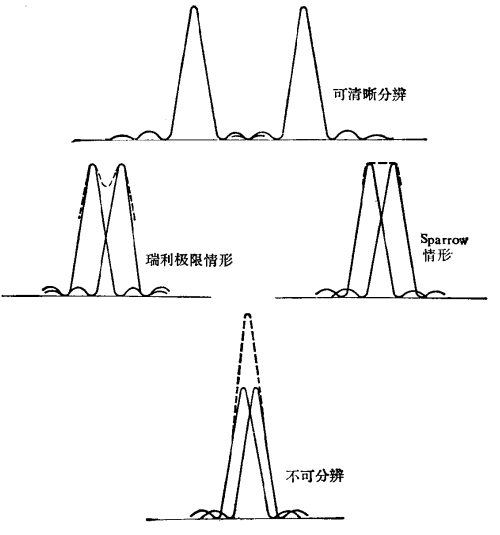
\includegraphics[width=12cm]{Diffraction_judge.png}
		\caption{重叠的两个点像}
		\label{figure_judge}
	\end{figure}

	利用色散的表达式,可以得到
	\begin{equation}
	(\Delta \theta)_{\min }=(\Delta \lambda)_{\min } m / a \cos \theta_{m}
	\end{equation}

\noindent 联立这两个式子可以得到:
\begin{equation}
	\begin{aligned}
	\lambda /(\Delta \lambda)_{\min }&=m N\\
	\mathscr{R}&=\frac{N a\left(\sin \theta_{m}-\sin \theta_{i}\right)}{\lambda}
	\end{aligned}
\end{equation}

\noindent 当光栅在自准直条件下使用时,得到最大的$ \mathscr{R} $值,此时
\begin{equation}
\mathscr{R}_{B}=\frac{2 N a \sin \theta_{i}}{\lambda}
\end{equation}

	考虑各级之间重叠的问题。如果波长在$ \lambda \rightarrow \lambda+\Delta \lambda $的两条谱线在相邻的$ (m+1) $和$ m $级中正好重叠在一起,那么
	\begin{equation}
	a\left(\sin \theta_{m}-\sin \theta_{i}\right)=(m+1) \lambda=m(\lambda+\Delta \lambda)
	\end{equation}
	
\noindent 这个波长差叫做自由频谱范围(free spectral range):
\begin{equation}
(\Delta \lambda)_{\text { fsr }}=\lambda / m
\end{equation}

	\section{菲涅耳衍射}
	\subsection{菲涅耳波带法}
	在夫琅禾费衍射的情况下,发射衍射的系统相对来说是小的,而观察点却离得非常远。在这种条件下,惠更斯-菲涅耳原理的一些有可能出问题的方面可以完全忽略过去,而当考虑近场区域时,就必须再回到惠更斯-菲涅耳原理本身上来了。
	
	如果把初波阵面上的每一点都想象成球面次级子波的一个持续不断的发射体,那如果每个子波向一切方向均匀地辐射,则除了产生一个向前进的波以外,还会出现一个背离波源后退的反向波,但实验中并没有发现这样一个波。为了修正这个问题,引入一个叫做\textbf{倾斜因子}的函数$ K(\theta) $,以描写次级发射的方向性。倾斜因子的正确表达式为
	\begin{equation}
	K(\theta)=\frac{1}{2}(1+\cos \theta)
	\end{equation}
	
\noindent 其中$ \theta $是同初波阵面的法线$ \mathbf{k} $的夹角,如下页顶图所示。

\noindent 这个函数在向前的方向上有极大值,并且没有后向波。

	我们现在来考察从点源$ S $发出的一个球面单色波的自由传播,球面相当于在某一任意时刻$ t^{\prime} $的初波阵面,它在$ t=0 $时从$ S $发出,这个 扰动的半径为$ \rho $,它可以用任何一个描述球面波的数学式子来表示,例如
	\begin{equation}
	E=\frac{\mathscr{E}_{0}}{\rho} \cos \left(\omega t^{\prime}-k \rho\right)
	\end{equation}
	
	我们可以把波阵面分为许多环状区域,各个区域的边界线对应于波阵面同一系列的球面的交线,这些球面的球心位于观察点,半径从观察点到衍射屏中心距离开始,每次增加半波长的距离。这些环状区域就是\textbf{菲涅耳波带}或\textbf{半周期波带}。
	
	由于波带上每个面元对观察点的贡献是复振幅,可以考虑无数矢量的叠加,最后正好形成一个半圆直径的合效果。
	
	\newpage
	\begin{figure}[htp]
		\centering
		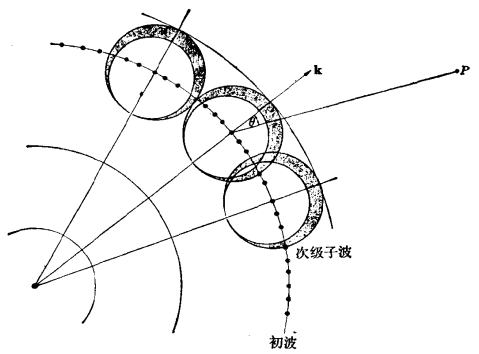
\includegraphics[width=12cm]{Diffraction_fei.png}
		\caption{次级子波}
		\label{figure_fei}
	\end{figure}

	\begin{figure}[ht]
		\centering
		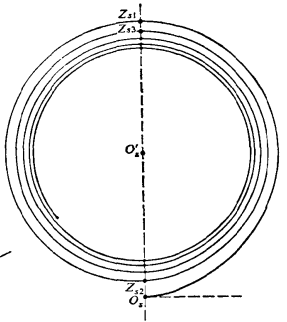
\includegraphics[width=8cm]{Diffraction_zhendong.png}
		\caption{振动曲线}
		\label{figure_zhendong}
	\end{figure}

	每个波带对观察点$ P $产生的电场贡献分别为$ E_{1}, E_{2}, E_{3}, \cdots $振幅只跟各波带到观察点的距离和倾斜因子有关(由于$ z_{1} \gg \lambda $,各波带面积可视为一样)。由于相邻波带的光程差为半波长,则相邻波带产生的复振幅分别为一正一负,认为相邻的三个复振幅之间的模大小相近,则可以近似为$ |\boldsymbol{E}_{n}| = \frac{|\boldsymbol{E}_{n-1}|}{2} + \frac{|\boldsymbol{E}_{n+1}|}{2} $。并且认为在$ n $足够大时,$ \boldsymbol{E}_{n-1} \approx \boldsymbol{E}_{n} $,得到
	\begin{equation}
	\boldsymbol{E} = \left \{
	\begin{aligned}
	\frac{|\boldsymbol{E}_{1}|}{2} &+ \frac{|\boldsymbol{E}_{n}|}{2}
	\\
	\frac{|\boldsymbol{E}_{1}|}{2} &+ \frac{|\boldsymbol{E}_{n-1}|}{2} - |\boldsymbol{E}|
	\end{aligned}
	\right.
	\end{equation}
	
\noindent 这个时候要考虑一个“骚操作”:虽然前面认为$ n $足够大,但依旧能够找到在这个条件下足够小的$ n $,使得不论$ n $为奇数还是偶数,都可以认为$ \boldsymbol{E}_{1} \approx \boldsymbol{E}_{n} $,由此可以得到
\begin{equation}
\boldsymbol{E} = \left \{
\begin{aligned}
\frac{|\boldsymbol{E}_{1}|}{2} &+ \frac{|\boldsymbol{E}_{n}|}{2} \approx |\boldsymbol{E}_{1}|
\\
\frac{|\boldsymbol{E}_{1}|}{2} &+ \frac{|\boldsymbol{E}_{n-1}|}{2} - |\boldsymbol{E}|
\end{aligned}
\right.
\end{equation}

	如果圆孔包含的波带数目很大,也即圆孔非常大时,可以得到$ |\tilde{\boldsymbol{E}}| = |\tilde{\boldsymbol{E}}_{1}|/2 $,表明这时观察点的复振幅等于第一个波带产生的复振幅的一半,强度为第一个波带片强度的$ \frac{1}{4} $。
	
	\subsection{圆孔和圆屏的衍射图样}
	\subsubsection{圆孔衍射}
	前面讨论了对于轴上观察点的圆孔衍射情况,与之类似,对于轴外点也可以使用类似的方法,只是这时波带对圆孔中心不再对称,一些序数较高的波带将部分地受到圆孔光屏的遮蔽,只有或多或少一部分在圆孔范围内露出来。这些波带在观察点产生的光强度,不仅取决于它们的数目,还取决于每个波带露出部分的面积。当离轴上点足够远时,圆孔范围内没有一个完整的波带了,并且奇数带和偶数带受光屏阻挡的情况差不多,因此这些地方都是暗的。
	
	\begin{figure}[H]
		\centering
		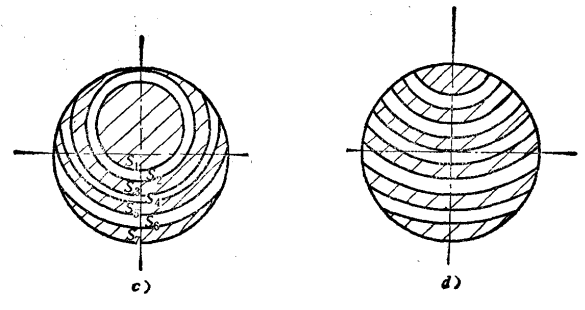
\includegraphics[width=12cm]{Diffraction_bodai.png}
		\caption{对应于不同考察点的波带形状}
		\label{figure_bodai}
		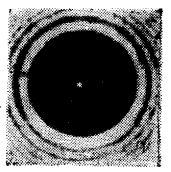
\includegraphics[width=6cm]{Diffraction_yuanping.png}
		\caption{菲涅耳圆屏衍射}
		\label{figure_yuanping}
	\end{figure}
	
	\subsubsection{圆屏衍射}
	同样采用波带法。全部波带在轴上点的复振幅应为第一波带产生的复振幅的一半,因此,可以断言轴上点总是亮点。对于轴外点,也可以使用类似的方法来讨论。轴外点随着离开轴心点的距离的增大,也会有光强大小的变化,因此,圆屏的衍射图样应该是:中心为亮点,周围有一些亮暗相间的圆形条纹。
	
	上面讨论是针对小圆屏而言的,当圆屏较大时,由于从圆屏边缘开始作出的第一波带对轴上点的作用甚微,所以其上的强度实际上接近于零,不再能看出是个亮点。
	
	\subsection{菲涅耳积分}
	对于圆形孔径的菲涅耳衍射,使用菲涅耳波带法可做定性和半定量的分析;而对于边缘都是平行于坐标轴的直边的孔径,如半平面屏、狭缝和矩孔时,可以直接应用菲涅耳衍射的计算公式进行计算。
	
	\subsubsection{直边的菲涅耳衍射}
	对于直边衍射,由于孔径与坐标轴平行,结果可以视为两个积分的乘积,各自有独立的积分限,由此得到
	\begin{equation}
		\tilde{\boldsymbol{E}}(\mu, v)= \frac{\exp (i k z_{1})}{2 i} \int_{\mu_{1}}^{\mu_{2}} \exp \left( i \frac{\pi \mu^{2}}{2}\right) \dif \mu \int_{v_{1}}^{v_{2}} \exp \left( i \frac{\pi v^{2}}{2}\right) \dif v
	\end{equation}
	
\noindent 其中,$ \mu = \sqrt{\frac{2}{\lambda z_{1}}} (x-x_{1}), v= \sqrt{\frac{2}{\lambda z_{1}}} (y-y_{1}) $.

	需要计算以下形式的积分
	\begin{equation}
		F(\omega) = \int_{0}^{\omega} \exp \left(i \frac{\pi t^{2}}{2} \right) \dif t
	\end{equation}
	
	这个积分叫做\textbf{菲涅耳积分},它包含有实部和虚部,即
	\begin{equation}
		F(\omega) = C(\omega) + i S(\omega) \label{equ_Fenier}
	\end{equation}
	
\noindent 其中,$ C(\omega) = \int_{0}^{\omega} \cos \frac{\pi t^{2}}{2} \dif t, S(\omega) = \int_{0}^{\omega} \sin \frac{\pi t^{2}}{2} \dif t $,分别称为\textbf{菲涅耳余弦积分、正弦积分}。以前者为横坐标,后者为纵坐标可得一曲线,被称为\textbf{科纽蜷线}。

\begin{figure}[H]
	\centering
	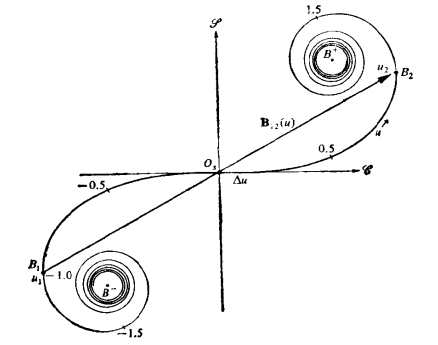
\includegraphics[width=12cm]{Diffraction_quanxian2.png}
	\caption{科纽蜷线1}
	\label{figure_quanxian1}
\end{figure}

\newpage
\begin{figure}[htp]
	\centering
	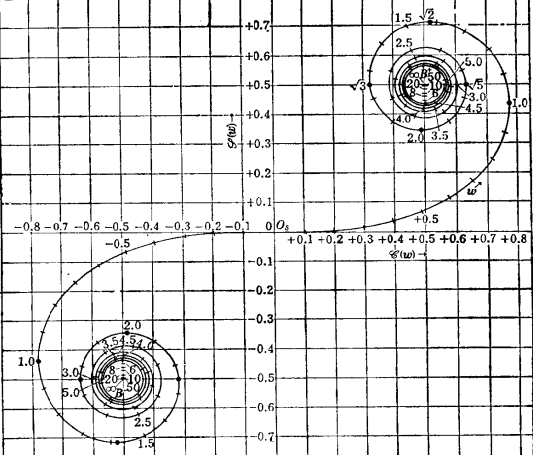
\includegraphics[width=12cm]{Diffraction_quanxian1.png}
	\caption{科纽蜷线2}
	\label{figure_quanxian2}
\end{figure}

	利用科纽蜷线求式\ref{equ_Fenier}的积分时很方便的,因为
	\begin{equation}
	\begin{aligned}
		\int_{\omega_{1}}^{\omega_{2}} \exp \left(i \frac{\pi t^{2}}{2}\right) \dif t &= \int_{0}^{\omega_{2}} \exp \left(i \frac{\pi t^{2}}{2}\right) \dif t - \int_{\omega_{0}}^{\omega_{1}} \exp \left(i \frac{\pi t^{2}}{2}\right) \dif t
		\\
		&= F(\omega_{2}) - F(\omega_{1})
	\end{aligned}
	\end{equation}
	
	\subsection{半平面屏、单缝和距孔菲涅耳衍射}
	对于半平面屏(也常称为\textbf{直边衍射}),容易得到
	\begin{equation}
	\tilde{\boldsymbol{E}}(x, y)=\frac{\exp \left(i k z_{1}\right)}{i \lambda z_{1}} \int_{0}^{\infty} \exp \left[\frac{i k}{2 z_{1}}\left(x-x_{1}\right)^{2}\right] d x_{1} \int_{-\infty}^{\infty} \exp \left[\frac{i k}{2 z_{1}}\left(y-y_{1}\right)^{2}\right] d y_{1}
	\end{equation}
	
\noindent 利用变量代换,可以得到
\begin{equation}
	\tilde{\boldsymbol{E}} (x,y) = =\frac{\exp \left(i k z_{1}\right)}{2 i}\left[F\left(x \sqrt{\frac{2}{\lambda z_{1}}}\right)-F(-\infty)\right][F(\infty)-F(-\infty)]
\end{equation}

\noindent 由于
\begin{equation}
	\begin{aligned}
F(\infty)=&\frac{\sqrt{2}}{2} \mathrm{e}^{\frac{\pi}{4}}=\frac{1}{2}(1+\mathrm{i}) 
\\ 
F(-\infty)=&-\frac{\sqrt{2}}{2} \mathrm{e}^{\frac{\pi}{4}}=-\frac{1}{2}(1+\mathrm{i})
	\end{aligned}
\end{equation}

\noindent 所以
\begin{equation}
\tilde{\boldsymbol{E}}(x, y)=\frac{(1+i) \exp \left(i k z_{1}\right)}{2 i}\left[F\left(x \sqrt{\frac{2}{\lambda z_{1}}}\right)-F(-\infty)\right]
\end{equation}

	注意当半平面屏不存在时,即波面无穷大时
	\begin{equation}
	\tilde{\boldsymbol{E}}=\tilde{\boldsymbol{E}}_{\infty}=\frac{\exp \left(\mathrm{i} k z_{1}\right)}{2 \mathrm{i}}(1+\mathrm{i})[F(\infty)-F(-\infty)]=\frac{\exp \left(\mathrm{i} k z_{1}\right)}{2 \mathrm{i}}(1+\mathrm{i})^{2}
	\end{equation}
	
	因此半平面屏的衍射公式又可以写作
	\begin{equation}
	\tilde{E}(x, y)=\frac{\tilde{E}_{\infty}}{(1+i)}\left[F\left(x \sqrt{\frac{2}{\lambda z_{1}}}\right)-F(-\infty)\right]
	\end{equation}
	
\noindent 由上式可知,衍射图样的复振幅和强度只随$ x $坐标变化,因此衍射图样是平行于$ y $轴的直线条纹。光强最大的点对应于$ \omega \approx 1.25 $,其光强值约为$ 1.37 I_{\infty} $,与之对应的是几何影区边缘旁的最亮的亮条纹。

	设单缝的宽度为$ a $,缝长$ \infty $,缝长方向平行于$ y_{1} $轴,则
	\begin{equation}
	\begin{aligned}
		\tilde{\boldsymbol{E}}(x, y)&=\frac{\exp \left(i k z_{1}\right)}{i \lambda z_{1}} \int_{-\frac{a}{2}}^{\frac{a}{2}} \exp \left[\frac{i k}{2 z_{1}}\left(x-x_{1}\right)^{2}\right] d x_{1} \int_{-\infty}^{\infty} \exp \left[\frac{i k}{2 z_{1}}\left(y-y_{1}\right)^{2}\right] d y_{1}
		\\
		&=\frac{(1+i) \exp \left(i k z_{1}\right)}{2 i}\left\{F\left[\left(x+\frac{a}{2}\right) \sqrt{\frac{2}{\lambda z_{1}}}\right]-F\left[\left(x-\frac{a}{2}\right) \sqrt{\frac{2}{\lambda z_{1}}}\right]\right\}
	\end{aligned}
	\end{equation}
	
\noindent 这就是单缝的菲涅耳衍射公式。它表示,单缝菲涅耳衍射同样可以利用菲涅耳积分和科纽蜷线来计算。对于一个特定的装置,大括号内的复数差可以表示为
\begin{equation}
	\Delta \omega=\omega_{2}-\omega_{1}=a \sqrt{\frac{2}{\lambda z_{1}}}
\end{equation}

\noindent 是一个常数。这样一来,当矢量两端点在科纽蜷线上$ \omega = 0 $附近时(两端点位置取决于$ x $值,当$ x = 0 $时,两端点对称地位于原点两边),一般地矢量长度较大;而当矢量两端点离开原点,进入蜷线的蜷曲部分时,矢量长度较短。

	设矩孔在$ x_{1} $的方向宽度为$ a $,在$ y_{1} $方向的宽度为$ b $。选取矩孔中心为坐标原点,得到矩孔衍射公式
	
	\begin{equation}
	\begin{aligned}
	\tilde{\boldsymbol{E}}(x, y)&=\frac{\exp \left(i k z_{1}\right)}{i \lambda z_{1}} \int_{-\frac{a}{2}}^{\frac{\pi}{2}} \exp \left[\frac{i k}{2 z_{1}}\left(x-x_{1}\right)^{2}\right] d x_{1} \int_{-\frac{b}{2}}^{\frac{b}{2}} \exp \left[\frac{i k}{2 z_{1}}\left(y-y_{1}\right)^{2}\right] \mathrm{d} y_{1}
	\\
	&=\frac{\tilde{E}_{\infty}}{(1+i)^{2}}\left\{F\left[\left(x+\frac{a}{2}\right) \sqrt{\frac{2}{\lambda z_{1}}}\right]-F\left[\left(x-\frac{a}{2}\right) \sqrt{\frac{2}{\lambda z_{1}}}\right]\right\} \times 
	\\
	&\left\{F\left[\left(y+\frac{b}{2}\right) \sqrt{\frac{2}{\lambda z_{1}}}\right]-F\left[\left(y-\frac{b}{2}\right) \sqrt{\frac{2}{\lambda z_{1}}}\right]\right\}
	\end{aligned}
	\end{equation}
	
\noindent 这表明,矩形衍射图样的振幅(强度)分布是两个互相垂直的单缝衍射图样振幅(强度)分布的乘积。因此,矩形衍射图样的分析方法与单缝衍射图样的分析方法相同。
\end{document}
